\documentclass[conference]{IEEEtran}
\usepackage{enumitem}
\usepackage{amsmath}
\usepackage{cite}
\usepackage{graphicx}
\usepackage{float}
\graphicspath{ {./}{./images/} }

\title{PCA-Based Image Compression}

\author{
\IEEEauthorblockN{Owen Sowatzke}
\IEEEauthorblockA{\textit{Electrical Engineering Department} \\
\textit{University of Arizona}\\
Tucson, USA \\
osowatzke@arizona.edu}
\and
\IEEEauthorblockN{Scott Thoesen}
\IEEEauthorblockA{\textit{Electrical Engineering Department} \\
\textit{University of Arizona}\\
Tucson, USA \\
thoesens@arizona.edu}}

\begin{document}
    
	\maketitle
	\begin{abstract}
	% Add abstract here
	\end{abstract}

	\begin{IEEEkeywords}
	% Add keywords here
	\end{IEEEkeywords}

    \section{Introduction}
    This project aims to explore principle component analysis (PCA), its relationship to singular value decomposition (SVD), and its application to the field of image compression \cite{jaradet_svd_image_compression}. The topic of digital image compression has become more important than ever with the advent of smartphones and social media, with millions of images created, stored, transferred, and copied daily. Reducing the digital footprint of this data is therefore necessary to both satisfying end-user demands and decreasing the demand on limited computing and storage resources. Image compression is important to the authors due to both of their backgrounds being in signal processing and computational systems. Additionally, the authors find interest in the more generalized understanding of PCA as a tool for data analysis and dimensionality reduction. Image compression was selected for this project to visually demonstrate the connection that is made by PCA between real-world data and linear algebra.

    \section{Background}
    PCA was not explicitly covered in ECE 501b but its underlying machinery, the SVD was. An entire lecture was dedicated to covering the SVD, which is an accumulation of many core concepts learned throughout the semester. The SVD employs many linear algebra concepts including inner product spaces, the null space, injectivity and surjectivity, dimensionality, linear independence, bases, orthonormality, linear maps, eigenvalues and eigenvectors, adjoints of linear maps, square roots of linear maps, matrix representations of linear maps, matrix decomposition, diagonal matrices, square matrices, unitary and orthonormal matrices. These concepts will appear throughout this paper and are assumed to be known by means of ECE 501b lectures. External references will therefore not be provided since the implication is that relevent ECE 501b lectures serve as the references.

    \subsection{Motivation}
    Digital images are signals, or vectors, which means they can be represented in various ways on different bases. Any basis is a collection of linearly independent vectors or functions that completely describe the vector space in which they are defined. Vectors, or signals, can therefore be represented on a basis as a linear combination of the constituent basis vectors. This representation is shown in Equation \ref{eq:basisdef}

    \begin{equation}
        v = \sum_{i=1}^{n} a_i \mathbf{\phi}_{i}
    \label{eq:basisdef}
    \end{equation}

    where $v$ is a vector, $a_i$ is a scalar, $\mathbf{\phi}_{i}$ is a basis vector or basis function, and $n$ is the length of the basis.

    Vectors in one basis can be converted to another by means of a linear transformation. Inverse operations also exist. Additionally, where a signal tends to be dense and feature rich in one basis, it is often sparse or compact in another. When a basis is identified such that a sparse or compact representation is possible, content that contains little to no information about the signal can be readily discarded. This leads to the intuition that signals are \textit{compressible}.

    Many compression techniques exist and fall into one of two categories: lossy and lossless. Lossless compression is concerned with the reduction of data size while maintaining the capacity to  completely recover the signal without degradation. Lossy compression concedes a level of irreversible degradation upon decompression. PCA-based compression is a lossy technique. Examples of other lossy compression schemes are JPEG, which employs the discrete cosine transform (DCT), and JPEG2000, which uses a wavelet transform \cite{jpeg_compression}\cite{jpeg2000_compression}.
    
    Under special considerations, information lost during lossy compression does not imply a reduction of image quality. For example, the chief premise behind JPEG compression is the fact that the human visual system cannot perceive high spatial frequencies beyond a certain limit. When the DCT of an image is computed, coefficients corresponding to frequency components beyond a certain threshold are discarded. The remaining lower-frequency components are retained and the image has been compressed. The decompressed image, obtained by an inverse DCT, is then indistinguishable from the original to a human observer.

    The DCT and other transforms involve bases that are independent of the data being transformed. This often leads to inefficient representations of a signal, and thus poor compressibility. Where a dense signal may appear to be sparse or compact when transformed to a certain basis, a different signal can remain dense or broadly distributed under the same transformation. JPEG exhibits this behavior when compressing natural images, such as a scene of trees, versus virtual images, such as a computer-generated graphic.
    
    SVD-, or PCA-, representation is a basis that is learned from the data itself. The basis vectors come from the structure of the signal and consequently form a more efficient representation. As will be shown in the Results section of this paper, this representation is also compact.
    
    \subsection{Singular Value Decomposition}
    The Singular Value Decomposition Theorem states that for any matrix $\mathbf{A} \in \mathbf{R}^{n \times n}$, a unique representation of the form shown in Equation \ref{eq:svddef} exists.

    \begin{equation}
        \mathbf{A} = \mathbf{U\Sigma }{\mathbf{V}^T}
    \label{eq:svddef}
    \end{equation}

    where $\mathbf{U} \in \mathbf{R}^{m \times m}$ and $\mathbf{V} \in \mathbf{R}^{n \times n}$ are square unitary
    matrices whose columns represent the left singular vectors and right singular vectors, respectively, and $\mathbf{\Sigma} \in \mathbf{R}^{m \times n}$ is a matrix of zeros except for the elements on the main diagonal which are the singular values. $m$ does not necessarily equal $n$. The singular values of $\mathbf{A}$ are always non-negative and real. When $\mathbf{A}$ is a real matrix, $\mathbf{U}$ and $\mathbf{V}$ are real and therefore orthonormal.

    A literal interpretation of the SVD is the action taken by a linear map split into three discrete operations. The first operation performs a rotation of a vector onto an orthonormal basis in the domain of the map. The second operation simultaneously scales the vector and potentially changes dimensionality. The final operation is a rotation onto an orthonormal basis in the co-domain of the map.

    The SVD is a generalized analog of the eigendecomposition of a matrix, which is a result of the Spectral Theorem for certain linear operators, or square matrices. The eigenvectors of a full-rank normal matrix, found through eigendecomposition, form an orthonormal basis on the inner product space of the matrix called an eigenbasis. Thus, any vector in the inner product space can be represented completely and uniquely as an appropriate scaling of the eigenbasis vectors. The vectors of an eigenbasis are also called the modes of the matrix. The magnitude of the eigenvalue associated with each mode determines the relative importance, or significance, of the mode in the composition of the matrix. Modes with higher importance, or larger eigenvalues, contain more pertinent information about the matrix than modes with smaller eigenvalues. Analogously, the right singular vectors of any matrix represent the modes of the matrix in the domain and the left singular vectors represent the modes in the co-domain. The magnitudes of the singular values determine the relative joint-importance, or joint-significance, of the associated left and right singular vectors in representing the matrix.

    Computing the SVD of a matrix $\mathbf{A}$ involves computing the eigendecomposition of both the row-wise autocorrelation matrix, $\mathbf{AA}^T$, and the column-wise autocorrelation matrix, $\mathbf{A}^T\mathbf{A}$. Both autocorrelation matrices are at least positive semi-definite which means unique eigendecompostions exist. Both decompositions are defined according to Equations \ref{eq:aatranspose} and \ref{eq:atransposea}

    \begin{equation}
         \mathbf{AA}^{T} = \mathbf{U\Lambda}\mathbf{U}^T
    \label{eq:aatranspose}
    \end{equation}

    \begin{equation}
         \mathbf{A}^T\mathbf{A} = \mathbf{V\Delta}\mathbf{V}^T
    \label{eq:atransposea}
    \end{equation}
    
    where $\mathbf{\Lambda} \in \mathbf{R}^{m \times m}$ is a diagonal matrix containing the eigenvalues of $\mathbf{AA}^{T}$, and $\mathbf{\Delta} \in \mathbf{R}^{n \times n}$ is a diagonal matrix containing the eigenvalues of $\mathbf{A}^T\mathbf{A}$. The non-zero elements of $\mathbf{\Lambda}$ are the same as the non-zero elements of $\mathbf{\Delta}$ and are equal to the squares of the singular values of $\mathbf{A}$. These eigenvalues are positive and real since the non-zero singular values are real.
    
    \subsection{Principle Component Analysis}
    
    Principle component analysis (PCA) re-expresses samples given in terms of one basis as linear combinations of new basis vectors \cite{shlens_2014_tutorial}. The new basis vectors are the principle components of the data set. They are chosen such the linear combination of basis vectors, used to write each sample, is largely dependent on the first basis vector and less dependent on subsequent basis vectors. This enables each sample of the data set to be approximated using fewer basis vectors. If the correct number of basis vectors are selected to approximate each sample, the data set can be compressed with minimal distortion.
    
    Denote each of the input sample as $\mathbf{x_i}$ and each of the principle components as $\mathbf{p_j}$, where $\mathbf{x_i}, \mathbf{p_j} \in \mathbf{R}^{m}$. If the principle components are constrained to orthonormal vectors, each input sample, $\mathbf{x_i}$ can be written as follows:
    %
    \begin{equation}
    		\mathbf{x_i} = \langle \mathbf{x_i}, \mathbf{p_1} \rangle \mathbf{p_1} + \cdots + \langle \mathbf{x_i}, \mathbf{p_m} \rangle \mathbf{p_m}
    		\label{eq:linear_combo_orthonormal_vectors}
    	\end{equation}
    	%
    	Let $\mathbf{y_i}$ be a vector of the scalars used to weight each of the principle components in equation (\ref{eq:linear_combo_orthonormal_vectors}). Then $\mathbf{y_i}$ can be written as follows:
    	%
    	\begin{equation}
        \mathbf{y_i} = \begin{bmatrix}
                        \langle \mathbf{x_i}, \mathbf{p_1} \rangle\\
                        \vdots \\
                        \langle \mathbf{x_i}, \mathbf{p_m}\rangle
                        \end{bmatrix}
    \end{equation}
    
    	Each $\mathbf{y_i}$ vector can be computed with a matrix equation. Let $\mathbf{X} \in \mathbf{R}^{m \times n}$ be the matrix formed by horizontally concatenating the column vectors $\mathbf{x_i}$.
    %
    \begin{equation}
    		\mathbf{X} = \begin{bmatrix}
    			\mathbf{x_1} & \mathbf{x_2} & \cdots & \mathbf{x_n}
    		\end{bmatrix}
    	\end{equation}
    	%
    	Similary, let $\mathbf{P} \in \mathbf{F}^{m \times m}$ be the matrix formed by vertically concatentating the row vectors $\mathbf{p_j}$.
	%
	\begin{equation}
    		\mathbf{P} = \begin{bmatrix}
    			\mathbf{p_1} \\ \mathbf{p_2} \\ \vdots \\ \mathbf{p_m}
    		\end{bmatrix}
    	\end{equation}
	%    	
    	Finally, let $\mathbf{Y} \in \mathbf{F}^{m \times n}$ be the matrix formed by horizontally concatenating the column vectors $\mathbf{y_i}$.
    	%
    \begin{equation}
    		\mathbf{Y} = \begin{bmatrix}
    			\mathbf{y_1} & \mathbf{y_2} & \cdots & \mathbf{y_n}
    		\end{bmatrix}
    	\end{equation}
    	%
    	Then, the following matrix equation will compute each $\mathbf{y_i}$ vector \cite{shlens_2014_tutorial}:
    	%
    	\begin{equation}
    		\mathbf{Y} = \mathbf{P}\mathbf{X}
    	\end{equation}

    	The principle components should be chosen such that each $\mathbf{y_i}$ can be approximated using a few of its starting elements, while setting the rest set to zero. In other words, the principle components should be chosen such that each $\mathbf{x_i}$ can be approximated by $\mathbf{\hat{x}_i}$, where 
    	%
    	\begin{equation}
 		\mathbf{\hat{x}_i} = \langle \mathbf{\hat{x}_i}, \mathbf{p_1} \rangle \mathbf{p_1} + \cdots + \langle \mathbf{\hat{x}_i}, \mathbf{p_k} \rangle \mathbf{p_k}
 	\end{equation}   	
    	%
    	for $k < m$. This is equivalent to selecting the first principle component to maximize the variance of $\mathbf{X}$ and selecting each subsequent principle component such that it is orthogonal to the previous principle components and maximizes the variance of $\mathbf{X}$ \cite{shlens_2014_tutorial}.
    	
    	The covariance matrix of $Y$ can be used to determine whether these conditions are met. It is defined as:
	%
	\begin{equation}
		\mathbf{C_y} = \frac{1}{n}{\mathbf{YY^T}}
	\end{equation} 
	%
	The principle components should minimize the redundancy of measurements, measured by the covariance (off-diagonal elements) and maximize the signal, measured by the variance (diagonal elements). Furthermore, the variances should be greatest for the first principle component and lower for each subsequent principle component. Therefore, the optimal covariance matrix will be diagonal, with the diagonal elements sorted in descending order \cite{shlens_2014_tutorial}.
	
	The principle components can be computed to provide the optimal covariance matrix. The covariance matrix can be rewritten as
	%
	\begin{equation}
		\mathbf{\mathbf{C_Y}} = {\mathbf{PC_XP^T}}
	\end{equation}
	%
	where $\mathbf{C_X}$ is the covariance matrix of $\mathbf{X}$ \cite{shlens_2014_tutorial}. If an eigen-decomposition of $\mathbf{C_X}$ is performed, the result will be
	%
	\begin{equation}
		\mathbf{C_X} = \mathbf{EDE^T}
	\end{equation}
	%
	where $\mathbf{E}$ is a matrix with columns that are the eigenvectors of $\mathbf{C_X}$ and $\mathbf{D}$ is a diagonal matrix with the eigenvalues of $\mathbf{C_X}$ on the diagonal. If $\mathbf{P} = \mathbf{E^{-1}} = \mathbf{E^T}$, the resulting covariance matrix $\mathbf{C_Y}$ will be diagonal and equivalent to $\mathbf{D}$. Therefore, the principle components should be the eigenvectors of $\mathbf{C_X}$, sorted based on their corresponding eigenvalues. I.e. \newline $\mathbf{p_1} = \mathbf{e_1}, ..., \mathbf{p_n} = \mathbf{e_n}$ for $\lambda_1 > \cdots > \lambda_n$. 
	
	SVD can also be used to find the principle components. Start by defining $\mathbf{A}$ such that
	%
	\begin{equation*}
		\mathbf{A} = \frac{1}{\sqrt{n}}\mathbf{X}
	\end{equation*}
	%
	Then, $\mathbf{AA^T} = \mathbf{C_X}$. Referring to Equation (\ref{eq:aatranspose}), the eigenvectors of $\mathbf{AA^T}$ are equivalent to the columns of $\mathbf{U}$. Furthermore, scaling the matrix $\mathbf{X}$ by $1/\sqrt{n}$ only scales the eigenvalues, $\Lambda$, but does not change the eigenvectors, $\mathbf{U}$. Therefore, an SVD can be performed directly $\mathbf{X}$ and the columns of the resulting $\mathbf{U}$ matrix will be the principle components.
    
    \subsection{Image Compression Using PCA} \label{pca_section}
    	
    	PCA can be used for image compression. Consider an grayscale image, which is a $m \times n$ matrix. 
    	%
    	\begin{equation}
    		\mathbf{X} = \begin{bmatrix}
    			x_{11} & x_{12} & \cdots & x_{1n} \\
    			x_{21} & x_{22} & \cdots & x_{2n} \\
    			\vdots & \vdots & \ddots & \vdots \\
    			x_{m1} & x_{m2} & \cdots & x_{mn}
    		\end{bmatrix}    			
    	\end{equation}
    	%
    	Each column of the above matrix can be treated as an input sample. PCA then attempts to find a better basis for each of these samples. As described above, the principles components are the columns of the $\mathbf{U}$ matrix that results from a SVD of the matrix $\mathbf{X}$.
	
	For $m < n$, the SVD output can be expanded as follows:
	
	\begin{equation}
		\begin{bmatrix}
			\mathbf{u_1} & \cdots & \mathbf{u_m}
		\end{bmatrix}\begin{bmatrix}
			\sigma_1 & 0 & \cdots & 0 & 0 & \cdots & 0\\
			0 & \sigma_2 & \cdots & 0 & 0 & \cdots & 0\\
			\vdots & \vdots & \ddots & \vdots & \vdots & \ddots & \vdots\\
			0 & 0 & \cdots & \sigma_m & 0 & \cdots & 0\\		
		\end{bmatrix}\begin{bmatrix}
			\mathbf{v_{1}^{T}}\\
			\vdots\\
			\mathbf{v_{n}^{T}}
		\end{bmatrix}		
	\end{equation}
	%
	where $\mathbf{u_i}$ are columns vectors of the $\mathbf{U}$ matrix, $\sigma_j$ are the singular values on the diagonal of the $\mathbf{\Sigma}$ matrix, and $\mathbf{v_k}$ are the column vectors of the $\mathbf{V}$ matrix.
	  
	Multiplying $\mathbf{\Sigma}$ with $\mathbf{V^T}$, the SVD output can be rewritten as follows:
	%
	\begin{equation}
		\begin{bmatrix}
			\mathbf{u_1} & \cdots & \mathbf{u_m}
		\end{bmatrix}\begin{bmatrix}
			\sigma_1v_{11} & \sigma_1v_{21} & \cdots & \sigma_1v_{n1}\\
			\sigma_2v_{12} & \sigma_1v_{22} & \cdots & \sigma_2v_{n2}\\
			\vdots & \vdots & \ddots & \vdots\\
			\sigma_mv_{1m} & \sigma_mv_{2m} & \cdots & \sigma_mv_{nm}
		\end{bmatrix}
	\end{equation}
	%
    	where $v_{ij}$ is the element of $\mathbf{V}$ in the ith column and jth row.
    	
    	The ith column of $\mathbf{X}$ matrix or the sample $\mathbf{x_i}$ can be written as follows:
	%
	\begin{equation*}
		\mathbf{x_i} = \sigma_1v_{i1}\mathbf{u_1} + \cdots \sigma_mv_{im}\mathbf{u_m}
	\end{equation*}   	
    	%
    	Recognizing that each $\mathbf{u_j}$ term is the principle component $\mathbf{p_j}$, the scalars $\sigma_jv_{ij}$ are the inner products $\langle \mathbf{x_i}, \mathbf{p_j}\rangle$. Therefore, the remaining SVD outputs, $\mathbf{\Sigma}$ and $\mathbf{V}$, can be used along with $\mathbf{U}$ to recreate each sample or column of the original image.  
    	
    	To perform compression, recognize that less important principle components can be discarded without significantly distorting the image.  Assume $r < m$ of the principle components are kept, and the rest are discarded. This is equivalent to keeping the first $r$ columns of the $\mathbf{U}$ matrix, the first $r$ rows and first $r$ columns of the $\mathbf{\Sigma}$ matrix, and the first $r$ columns of the $\mathbf{V}$ matrix. Because $\mathbf{\Sigma}$ is diagonal, storage can be further optimized by keep just the first $r$ diagonal elements of $\mathbf{\Sigma}$.
    	
    Note that the result above was derived using $m < n$. However, the result is similar for $n < m$. The only difference is that $r$ must be less than $n$ instead of $m$. Therefore, in general, the SVD output can be used to compress an image. The compressed image will consist of a matrix $\mathbf{\hat{U}} \in \mathbf{R}^{m \times r}$, a vector $\mathbf{\sigma} \in \mathbf{R}^{r}$, and a matrix $\mathbf{\hat{V}} \in \mathbf{R}^{n \times r}$. To reconstruct the image, form an $r \times r$ diagonal matrix $\mathbf{\hat{\Sigma}}$ using the vector $\mathbf{\sigma}$. Then, the reconstructed image $\mathbf{\hat{X}}$ is given by Equation \label{eq:imgrecon}

    \begin{equation}
        \mathbf{\hat{X}} = \mathbf{\hat{U}{\hat{\Sigma}}\hat{V}^T}
    \label{eq:imgrecon}
    \end{equation}
    \section{Results}

    The compression technique described in Section \ref{pca_section} is implemented in Matlab. The Matlab built-in image 'wagon.jpg' is used throughout this section as an example for both qualitative and quantitative analysis of the compression scheme. Qualitative analysis is performed through visual inspection of image quality after compression. Quantitative analysis is performed by examining the peak signal-to-noise ratio (PSNR) of the compressed image, compared to the original, uncompressed image.

    \subsection{Data}
    The Matlab built-in image 'wagon.jpg' is an 8-bit 1024x768 RGB image that contains three channels of red, green, and blue color data. The total uncompressed image size is 2,359,296 Bytes, or 2.25 MB.

    \subsection{Design}
    The compression engine works in four main steps, repeated for each of three color channels. The first step converts the image matrix of size $m \times n$ to a double precision floating point representation. The second step computes the mean value of the entire matrix and subtracts it from each element. The third step implements Matlab's built-in SVD function to calculate the $\mathbf{U}$, $\mathbf{\Sigma}$, and$\mathbf{V}$ matrices. The fourth step involves truncating the SVD by storing the first $r$ columns of the $\mathbf{U}$ and $\mathbf{V}$ matrices and the first $r$ elements of the trace of the $\mathbf{\Sigma}$ matrix. The matrix mean value is also stored.

    Decompression, or reconstruction, is performed in one step according to Equation \ref{eq:imgrecon}
    
    \subsection{Analysis}
    As mentioned in Section \ref{pca_section} every matrix can be decomposed into a linear combination of its modes. The relative importance, or significance, of a mode is determined by the magnitude of its associated singular value. A digital image is represented by a matrix and is therefore decomposed in the same way. In the context of image decomposition, the magnitude of each singular value determines the relative quantity of image information present in the respective modes.

	 \begin{figure}[t]
        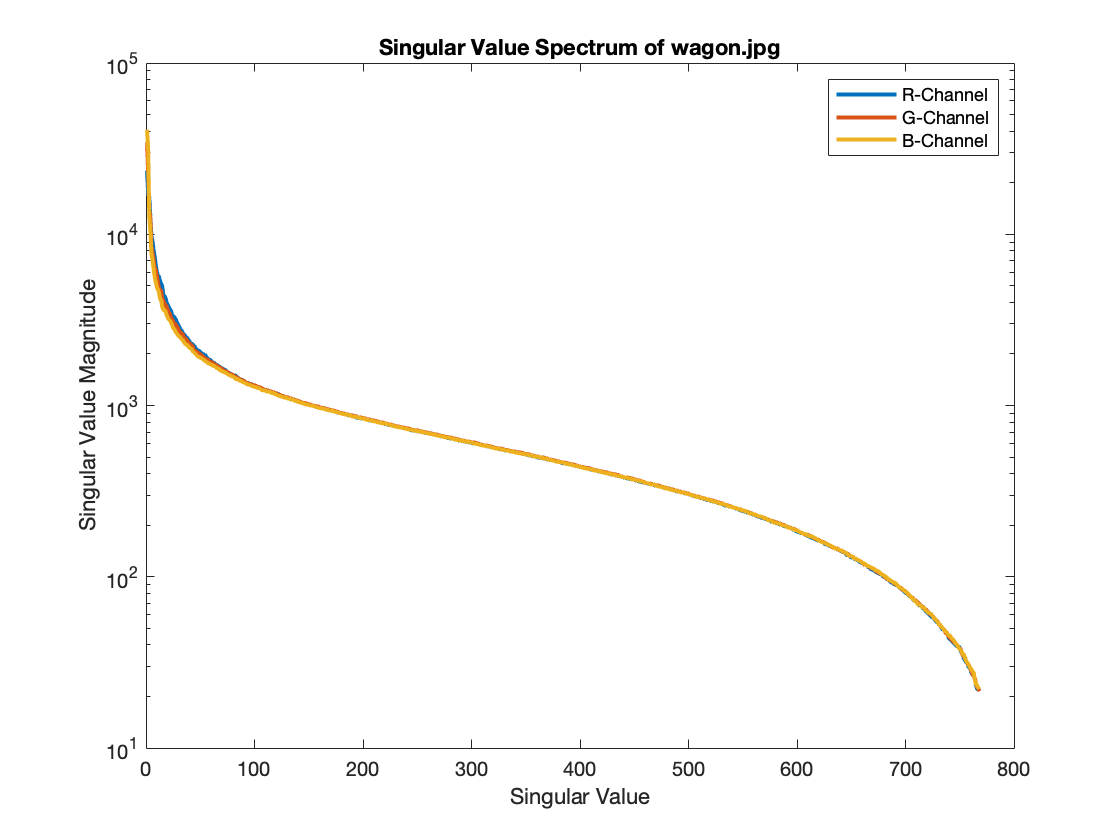
\includegraphics[width=0.5\textwidth]{svals_wagon_rgb}
        \caption{Singular Value Spectrum of wagon.jpg. The SVD is computed separately for the red (R), green (G), and blue (B) channels}
        \label{fig:svalplot}
    \end{figure}
    
	\begin{figure}[t]
        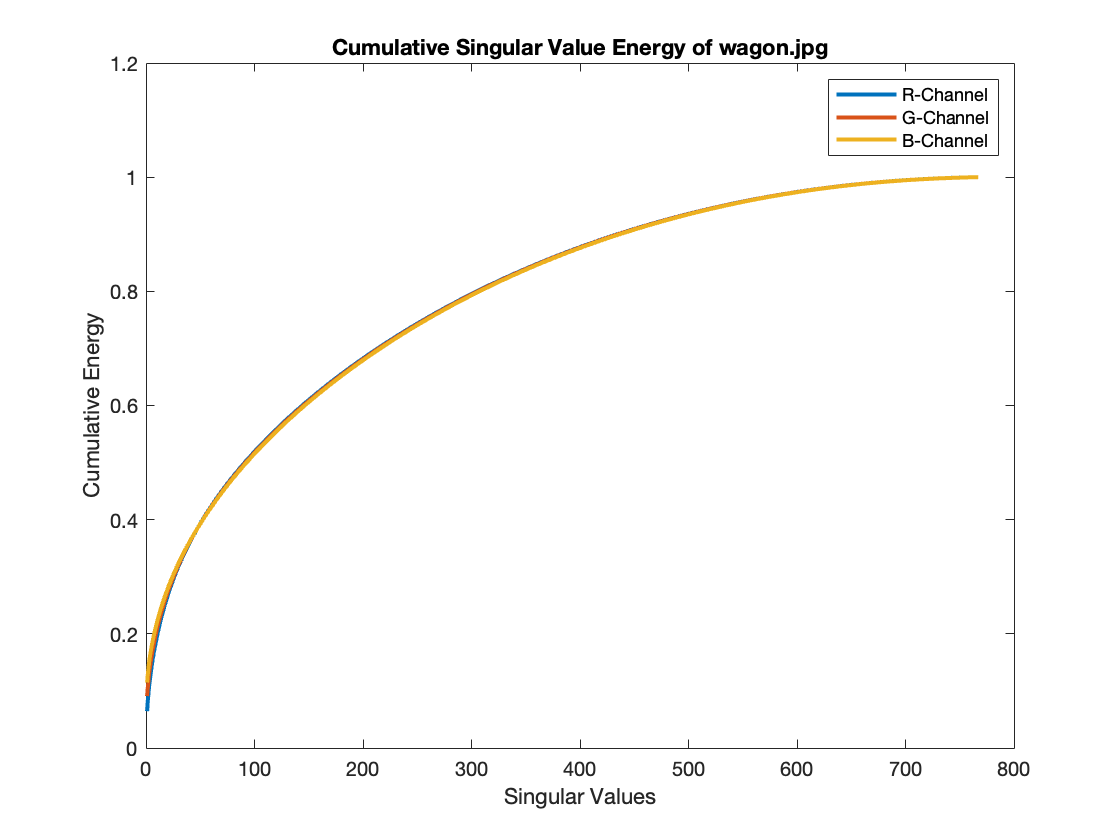
\includegraphics[width=0.5\textwidth]{sv_energy_wagon_rgb}
        \caption{Plot showing the cumulative energy of the singular values of wagon.jpg. Cumulative energy is computed separately for the red (R), green (G), and blue (B) channels}
        \label{fig:svalenergyplot}
    \end{figure}
    
    \begin{figure}[t]
        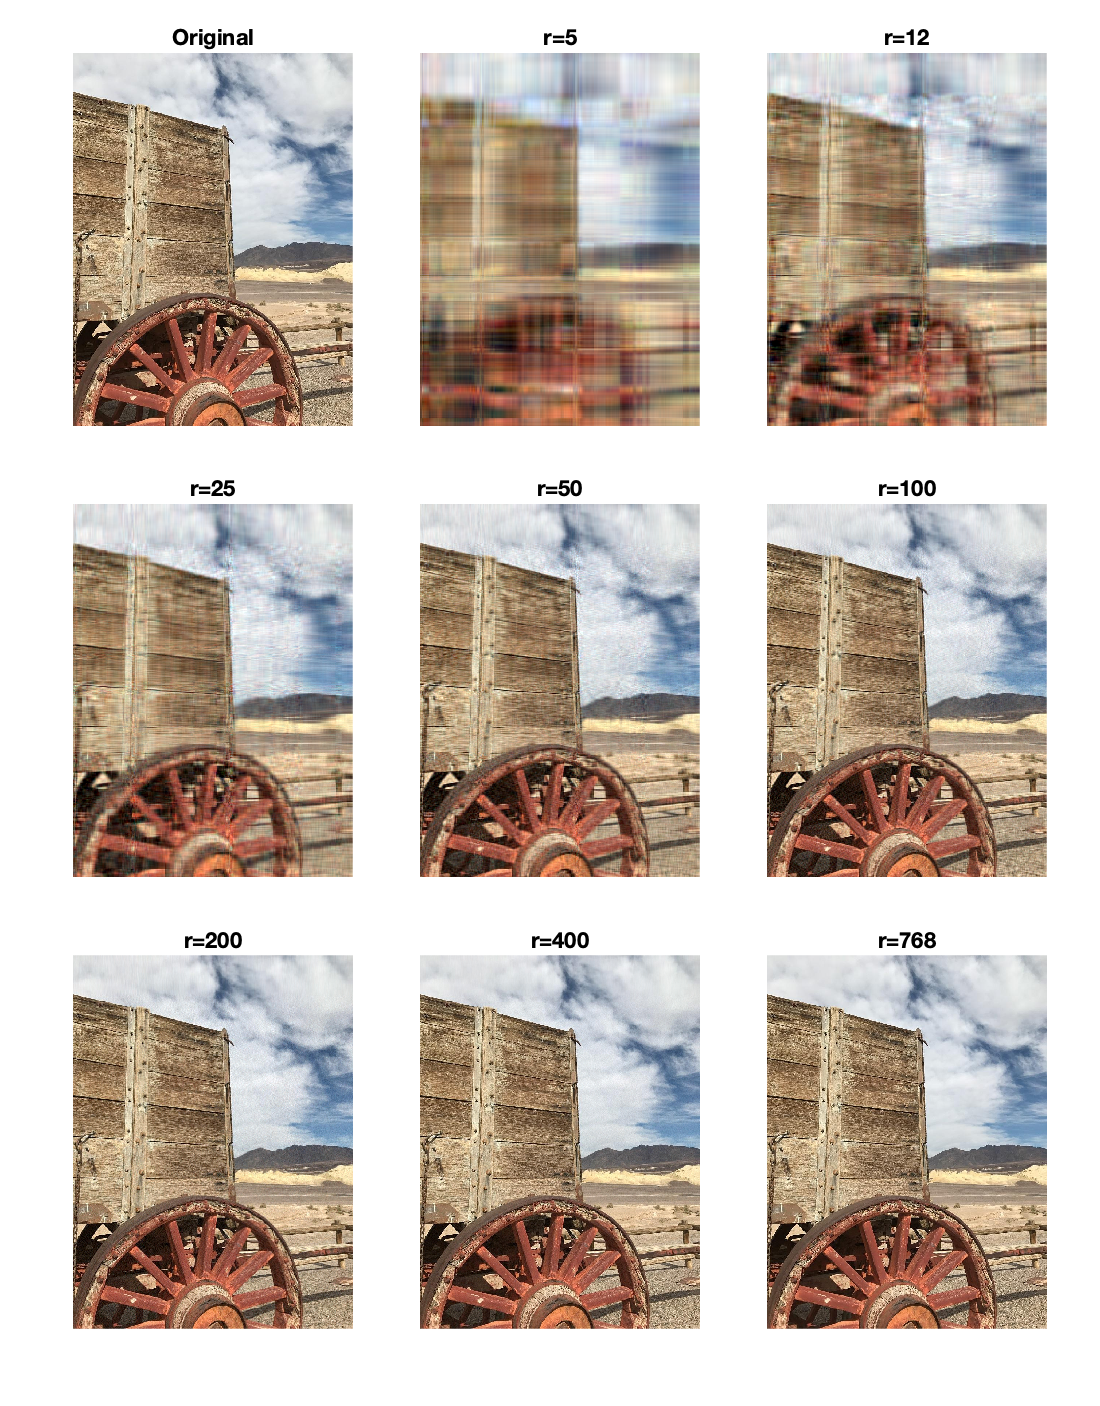
\includegraphics[width=0.5\textwidth]{show_different_r_wagon}
        \caption{Wagon wheel image using various numbers of representative modes}
        \label{fig:showwagondiffr}
    \end{figure}
    
    Shown in Figure \ref{fig:svalplot} is a plot of the singular values, also called the singular value spectrum, of the image wagon.jpg. Of particular note is the low number of large singular values, approximately 100-200, compared to the total of 768. This concentration of large singular values suggests the majority of the modes contain little relevant information about the image. Thus, removing these unimportant modes should agree with the intuition that images can be reduced in size while preserving the majority of the information content. Since the image is completely defined by the combination of all modes, the sum total of the singular values can be seen as a reasonable analog for the total information, or energy, contained in the image. Figure \ref{fig:svalenergyplot} shows the accumulation of energy as the number of modes representing the image increases from most to least significant. For example, to represent 80\% of the content of the image, the first 300 modes are needed.

    The effect of additional modes can be seen in Figure \ref{fig:showwagondiffr}. There are clear signs of distortion when the number of representative modes is low, in the range of 10-20, but distortion appears to fade as the number of modes reaches 200-400. According to the cumulative energy plot in Figure \ref{fig:svalenergyplot}, this level of compression retains 68\% to 88\% of the information content of the image. A more quantitative measure of compressed image quality is peak signal-to-noise ratio (PSNR), defined in Equation \ref{eq:psnr}

    \begin{equation}
    		PSNR = 10log_{10}(\frac{peakval^2}{MSE})
    \label{eq:psnr}
    \end{equation}

    where $peakval$ is the maximum representable value of the image's datatype - 8-bit integers in this example - and $MSE$ is the mean squared error between the compressed image and original, uncompressed image.

	\begin{figure}[t]
        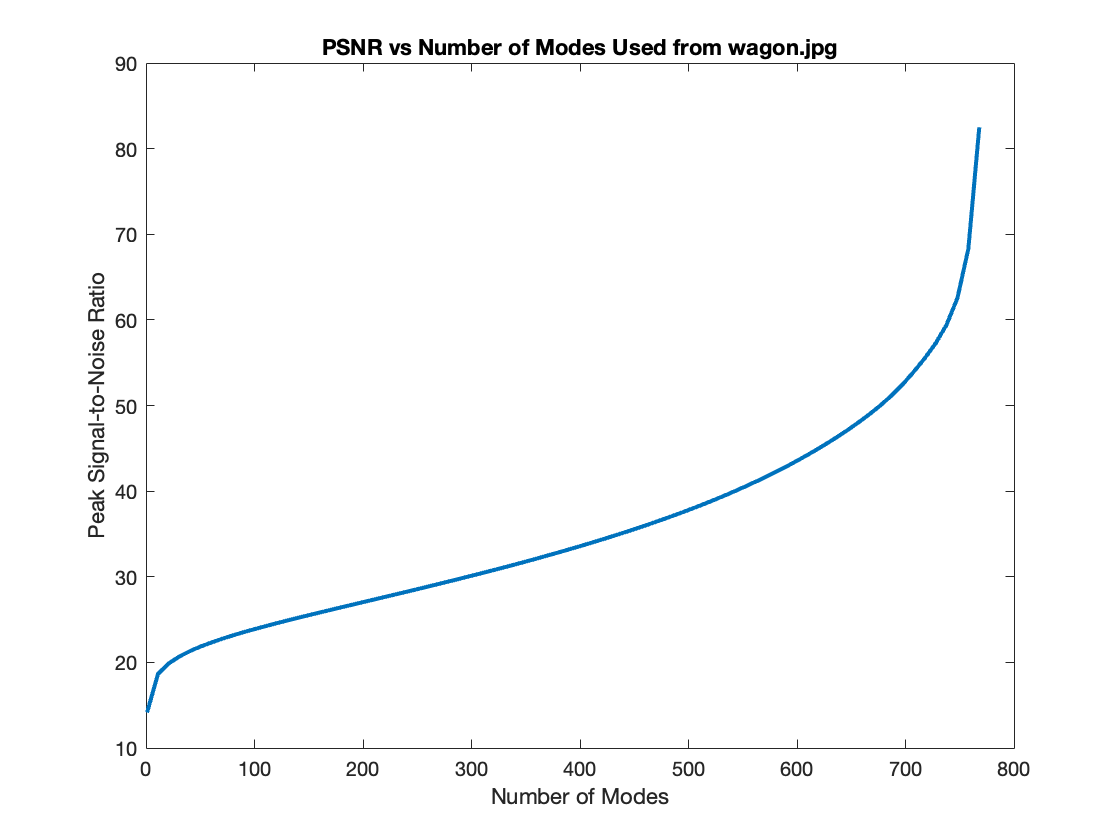
\includegraphics[width=0.5\textwidth]{snrvsr_wagon_rgb}
        \caption{Peak signal-to-noise ratio versus total number of modes}
        \label{fig:psnrvsr_wagon}
    \end{figure}
    
    Figure \ref{fig:psnrvsr_wagon} shows a plot of PSNR versus number of modes representing the wagon image. PSNR rises rapidly for the first few modes, then steadily for the total number of modes ranging from ~100 to ~550, then rapidly again as the decompressed image approaches the true image in value. Theoretical PSNR for a perfect reconstruction is infinity but that unlikely to be achieved due to quantization error. According to \cite{psnr_quality} typical PSNR values for a high quality lossy reconstruction of an 8-bit image are 30-50dB. This agrees with our quantitative result which shows a PSNR range of 27-34dB for 200-400 modes, as well as our qualitative result which shows virtually no difference between a 200-400 mode image and the original.

    \begin{figure}[t]
    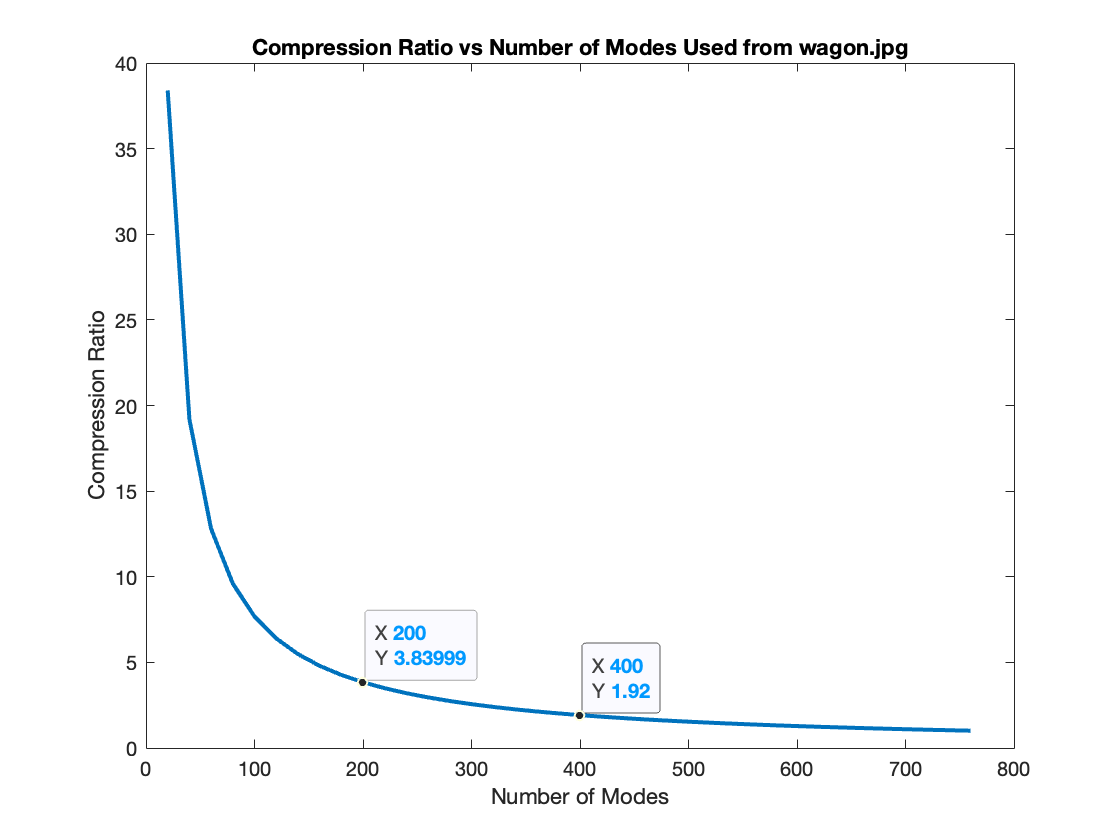
\includegraphics[width=0.5\textwidth]{comprVsModes_rgb}
    \caption{Compression ratio versus total number of modes}
    \label{fig:comprvsr}
    \end{figure}
    
    Retaining the first 200-400 modes would suggest, from a subjective perspective, that the image can be reduced in size by a factor of 1.92 to 3.84. According to the plot in Figure \ref{fig:comprvsr}, the computed compression ratio for 100-200 modes is indeed between 1.92 and 3.84. This direct relationship suggests compression ratio is simply a function of number of modes.

    % Add comments about the differences between the Y and Cb/Cr curves?

    %Using the 25,000,000,000 Eigenvector paper as a guide, develop some exercises, questions, analysis, or examples that were inspired or motivated by your project. For example, what assumptions were made in your project material? What if certain assumptions are neglected or do not exist? Can you provide analysis that supplements the analysis in the selected project material Or, can you provide analysis that extends the analysis in the project material You might also develop numerical examples that help to provide insight into the ideas discussed in the selected material or that demonstrate the application of the theory in your project. The example you create might consist of a MATLAB simulation or MATLAB analysis.
    \section{Conclusion}

    In this paper we were able to show that the SVD and concepts from PCA could be implemented from scratch and used to solve the problem of image compression. A qualitative analysis by visual inspection and quantitative analysis using PSNR showed that an image can be compressed by a factor of 1.92 to 3.84 without a perceptive loss of quality. Compression is achieved by preserving the first 200-400 modes, or principle components, out of a total of 768. The PSNR of the compressed image ranges from 27dB to 34dB which is comparable to a high quality reconstruction. The implemented process and results are in agreement with the chief material in \cite{jaradet_svd_image_compression}.
    
    Future work would involve modifying the example to perform compression on the YCbCr color space as described in \cite{xu_color_conversion}. Where the singular value spectrum of an RGB image has the same shape for all three channels, the spectra for chrominance channels are more compact than that of the luminance channel. This leads to the possibility that further compression can be achieved by using less Cb and Cr modes than Y modes.

    This project was an exercise in understanding the intricacies of the SVD and PCA, and the connection between them. Understanding these concepts requires a deep understanding of most of the topics covered in ECE 501b. By choosing this topic, one is forced to review all the fundamentals that are taught in class.

    %Provide a summary and conclusion section in the report. How well did your example correlate or explain the concepts in the selected material? How would you modify your example to make it better? How did your selected project enhance your understanding of ECE 501b material?

    \nocite{jaradet_svd_image_compression}
    \nocite{shlens_2014_tutorial}
    \nocite{omar_image_compression}
    \nocite{xu_color_conversion}
    %\newpage
    \bibliography{sources}{}
    \bibliographystyle{ieeetr}
\end{document}
